%%%%%%%%%%%%%%%%%%%%%%%%%%%%%%%%%%%%%%%%%
% University/School Laboratory Report
% LaTeX Template
% Version 3.1 (25/3/14)
%
% This template has been downloaded from:
% http://www.LaTeXTemplates.com
%
% Original author:
% Linux and Unix Users Group at Virginia Tech Wiki 
% (https://vtluug.org/wiki/Example_LaTeX_chem_lab_report)
%
% License:
% CC BY-NC-SA 3.0 (http://creativecommons.org/licenses/by-nc-sa/3.0/)
%
%%%%%%%%%%%%%%%%%%%%%%%%%%%%%%%%%%%%%%%%%

%----------------------------------------------------------------------------------------
%	PACKAGES AND DOCUMENT CONFIGURATIONS
%----------------------------------------------------------------------------------------

\documentclass{article}

\usepackage[version=3]{mhchem} % Package for chemical equation typesetting
\usepackage{siunitx} % Provides the \SI{}{} and \si{} command for typesetting SI units
\usepackage{graphicx} % Required for the inclusion of images
\usepackage{natbib} % Required to change bibliography style to APA
\usepackage{amsmath} % Required for some math elements 

\setlength\parindent{0pt} % Removes all indentation from paragraphs

\renewcommand{\labelenumi}{\alph{enumi}.} % Make numbering in the enumerate environment by letter rather than number (e.g. section 6)

%\usepackage{times} % Uncomment to use the Times New Roman font

%----------------------------------------------------------------------------------------
%	DOCUMENT INFORMATION
%----------------------------------------------------------------------------------------

\title{Connettore Publish-Subscribe Content-Based adeguato ad ambiente Mobile per mezzo di politiche adattative } % Title

\author{Stefano \textsc{Agostini} Matricola: 0234240 \\ Paolo \textsc{Salom\'e} Matricola: 1234567 \\ Alessandro \textsc{Valenti} Matricola: 0228709} % Author name

\date{\today} % Date for the report

\begin{document}

\maketitle % Insert the title, author and date

%\begin{center}
%\begin{tabular}{l r}
%Date Performed: & January 1, 2012 \\ % Date the experiment was performed
%Partners: & James Smith \\ % Partner names
%& Mary Smith \\
%Instructor: & Professor Smith % Instructor/supervisor
%\end{tabular}
%\end{center}

% If you wish to include an abstract, uncomment the lines below
% \begin{abstract}
% Abstract text
% \end{abstract}

%----------------------------------------------------------------------------------------
%	SECTION 1
%----------------------------------------------------------------------------------------

\section{Introduzione}

Il connettore \textit{Publish-Subscribe} presenta caratteristiche interessanti per sistemi caratterizzati da una elevata dinamicit\'a, grazie all'elevato livello di disaccoppiamento che \'e in grado di garantire tra componenti. I componenti coinvolti nell'interazione, per mezzo del connettore, sono i \textit{produttori} e i \textit{consumatori} di determinati eventi generabili. Un evento \'e caratterizzato dal cosidetto \textit{topic} che rappresenta il suo argomento d'appartenenza al quale un \textit{consumatore} pu\'o sottoscriversi se interessato a tale classe di informazioni; il \textit{produttore} a sua volta pu\'o pubblicare eventi associati ad un determinato \textit{topic}. Nello specifico \'e possibile caratterizzare un determinato evento (dopo averlo associato ad un \textit{topic}) in base al suo contenuto utilizzando la politica del tipo \textit{content-based}. Tale modalit\'a di sottoscrizione viene realizzata specificando un filtro e di conseguenza favorisce la riduzione del carico di eventi recapitati ai \textit{consumatori}. Il connettore realizzato si presta all'utilizzo in ambiente mobile in quanto garantisce un alto grado di disaccoppiamento, garantendo uno scambio affidabile di messaggi tra le entit\'a coinvolte. Tuttavia ci siamo posti come obiettivo quello di aggiungere a tale sistema politiche adattative che tengano conto delle limitate risorse energetiche e computazionali a disposizione dei nodi mobili, continuando a garantire uno scambio affidabile di messaggi tra le entit\'a attraverso il connettore.
Intuendo un legame funzionale tra consumo energetico e traffico generato dal nodo mobile, abbiamo compiuto uno studio statistico per avallare la nostra ipotesi che si \'e rivelato soddisfacente: pertanto abbiamo potuto realizzare un modello matematico finale. 
La nostra politica adattativa ci permette di controllare il tasso di consumo energetico controllando direttamente la frequenza di interazione del nodo mobile con la rete, gestendo, tramite un monitoraggio continuo dello stato della batteria, le risorse limitate del dispositivo. % scrivere in una frase che il nostro sistema implementa mape?

\section{Obiettivi}

L'obiettivo \'e quello di realizzare un connettore \textit{Publish-Subscribe} in modalit\'a \textit{content-based} ed adattarlo ad ambiente mobile. Nel dettaglio il nostro sistema deve essere costituito da nodi mobili che possono assumere il ruolo di \textit{consumatore o produttore} e dal connettore che deve comporsi delle seguenti entit\'a:

\begin{itemize}
\item{\textit{Event-Service}, il quale si preoccupa di gestire gli eventi generati e di recapitare notifiche}
\item{\textit{Filter-Service}, il quale realizza la modalit\'a di sottoscrizione \textit{content-based}}
\end{itemize}

Si vuole inoltre adattare tale sistema ad ambiente mobile mediante una politica che abbia come scopo quello di monitorare e controllare:

\begin{itemize}
\item{\textit{Il consumo energetico}}
\item{\textit{Il traffico generato} nell'interazione tra nodo mobile e connettore}
\end{itemize}

\section{Architettura generale}

Il sistema si basa fondamentalmente su un'architettura centralizzata. Infatti il connettore \textit{Publish-Subscribe} si compone di un server che svolge sia la funzione di \textit{Event-Service} che la funzione di \textit{Filter-Service}. I client non interagiscono direttamente con il connettore ma scambiano messaggi mediante delle code che implementano il paradigma di interazione \textit{message queueing}. Tale paradigma offre dei vantaggi in termini di disaccoppiamento spaziale e temporale, garantendo la possibilit\'a al client di potersi disattivare o spegnere immantinentemente una volta inoltrato un messaggio.
\\
Il server gestisce, tramite una \textit{database non relazionale} distribuito, la persistenza delle informazioni indispensabili per il corretto funzionamento del sistema dal punto di vista dei client, ovvero

\begin{itemize}
\item{\textit{Topic}}
\item{\textit{Sottoscrizioni e Filtri}}
\end{itemize}

I nodi mobili, cos\'i come il server, gestiscono la persistenza in locale di alcune informazioni attraverso un \textit{database relazionale}. Tali informazioni sono i \textit{topic} al momento disponibili nel sistema, le \textit{notifiche} in ingresso, le \textit{sottoscrizioni} effettuate con i relativi \textit{topic e filtri}. Il client attraverso procedure interne effettua, periodicamente,  un'operazione di \textit{pull} sulla coda per poter aggiornare i dati relativi alle notifiche ad esso destinate. Analogamente richiede al server la lista dei \textit{topic} disponibili per aggiornare le sue informazioni locali. Tutto ci\'o viene attuato per promuovere un utilizzo offline dell'applicazione in caso di disconnessione, scenario possibile nell'ambito dei sistemi mobili.\\
Di seguito illustriamo l'architettura attraverso uno schema in \figurename{~\ref{fig:Architettura}}.

\begin{figure}[h]
\begin{center}
\centering
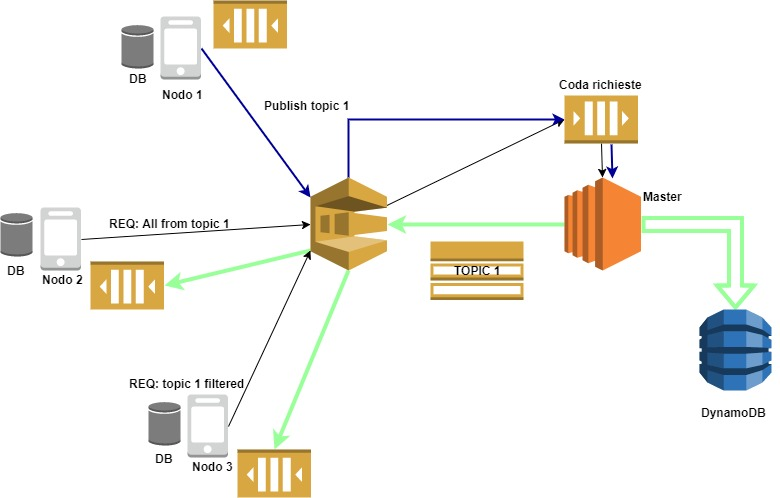
\includegraphics[width=1.25\textwidth]{architettura.jpg} % Include the image placeholder.png
\caption{Architettura}
\label{fig:Architettura}
\end{center}
\end{figure}

\subsection{Servizi Cloud}

Come \textit{Cloud Provider} \'e stato scelto \textit{Amazon AWS}. I servizi utilizzati per l'implementazione del connettore sono:

\begin{itemize}
\item{\textbf{Amazon EC2}: servizio \textit{IaaS} sfruttato per la realizzazione del nodo master che identifica il server dell'architettura. Svolge il ruolo di \textit{Event-Service e Filter-Service} nonch\'e di gestore del \textit{database NoSQL}. Per la comunicazione con i nodi client interagisce con le code del servizio \textit{Amazon SQS}}
\item{\textbf{Amazon SQS}: è un servizio di accodamento di messaggi distribuito che disaccoppia completamente i componenti dell'architettura. In tal modo semplifica e riduce i costi del coordinamento dei componenti stessi. Offre un \textit{throughput} elevato e \textit{tunable}, un ordinamento semplificato e distribuzione di tipo \textit{at-least-once}. In generale \'e possibile impostare un algoritmo di \textit{scheduling} dei messaggi: nel nostro caso \'e stato utilizzato l'algoritmo \textit{FIFO}}
\item{\textbf{Amazon DynamoDB}}
\end{itemize}

\subsection{Piattaforma Client}

\subsection{Interazione dei componenti}
 
%----------------------------------------------------------------------------------------
%	SECTION 2
%----------------------------------------------------------------------------------------

\section{Experimental Data}

\begin{tabular}{ll}
Mass of empty crucible & \SI{7.28}{\gram}\\
Mass of crucible and magnesium before heating & \SI{8.59}{\gram}\\
Mass of crucible and magnesium oxide after heating & \SI{9.46}{\gram}\\
Balance used & \#4\\
Magnesium from sample bottle & \#1
\end{tabular}

%----------------------------------------------------------------------------------------
%	SECTION 3
%----------------------------------------------------------------------------------------

\section{Sample Calculation}

\begin{tabular}{ll}
Mass of magnesium metal & = \SI{8.59}{\gram} - \SI{7.28}{\gram}\\
& = \SI{1.31}{\gram}\\
Mass of magnesium oxide & = \SI{9.46}{\gram} - \SI{7.28}{\gram}\\
& = \SI{2.18}{\gram}\\
Mass of oxygen & = \SI{2.18}{\gram} - \SI{1.31}{\gram}\\
& = \SI{0.87}{\gram}
\end{tabular}

Because of this reaction, the required ratio is the atomic weight of magnesium: \SI{16.00}{\gram} of oxygen as experimental mass of Mg: experimental mass of oxygen or $\frac{x}{1.31}=\frac{16}{0.87}$ from which, $M_{\ce{Mg}} = 16.00 \times \frac{1.31}{0.87} = 24.1 = \SI{24}{\gram\per\mole}$ (to two significant figures).

%----------------------------------------------------------------------------------------
%	SECTION 4
%----------------------------------------------------------------------------------------

\section{Results and Conclusions}

The atomic weight of magnesium is concluded to be \SI{24}{\gram\per\mol}, as determined by the stoichiometry of its chemical combination with oxygen. This result is in agreement with the accepted value.

\begin{figure}[h]
\begin{center}

\includegraphics[width=0.65\textwidth]{placeholder} % Include the image placeholder.png
\caption{Figure caption.}
\end{center}
\end{figure}

%----------------------------------------------------------------------------------------
%	SECTION 5
%----------------------------------------------------------------------------------------

\section{Discussion of Experimental Uncertainty}

The accepted value (periodic table) is \SI{24.3}{\gram\per\mole} \cite{Smith:2012qr}. The percentage discrepancy between the accepted value and the result obtained here is 1.3\%. Because only a single measurement was made, it is not possible to calculate an estimated standard deviation.

The most obvious source of experimental uncertainty is the limited precision of the balance. Other potential sources of experimental uncertainty are: the reaction might not be complete; if not enough time was allowed for total oxidation, less than complete oxidation of the magnesium might have, in part, reacted with nitrogen in the air (incorrect reaction); the magnesium oxide might have absorbed water from the air, and thus weigh ``too much." Because the result obtained is close to the accepted value it is possible that some of these experimental uncertainties have fortuitously cancelled one another.

%----------------------------------------------------------------------------------------
%	SECTION 6
%----------------------------------------------------------------------------------------

\section{Answers to Definitions}

\begin{enumerate}
\begin{item}
The \emph{atomic weight of an element} is the relative weight of one of its atoms compared to C-12 with a weight of 12.0000000$\ldots$, hydrogen with a weight of 1.008, to oxygen with a weight of 16.00. Atomic weight is also the average weight of all the atoms of that element as they occur in nature.
\end{item}
\begin{item}
The \emph{units of atomic weight} are two-fold, with an identical numerical value. They are g/mole of atoms (or just g/mol) or amu/atom.
\end{item}
\begin{item}
\emph{Percentage discrepancy} between an accepted (literature) value and an experimental value is
\begin{equation*}
\frac{\mathrm{experimental\;result} - \mathrm{accepted\;result}}{\mathrm{accepted\;result}}
\end{equation*}
\end{item}
\end{enumerate}

%----------------------------------------------------------------------------------------
%	BIBLIOGRAPHY
%----------------------------------------------------------------------------------------

\bibliographystyle{apalike}

\bibliography{sample}

%----------------------------------------------------------------------------------------


\end{document}